
\chapter{Validation and Results}
\label{cha:validationresults}

To validate our solution, we implemented a simple distributed application using a traditional approach and an approach that makes use of our solution, which we shall call the by-move solution. The application is based on a banking system using a microservices-like architecture. In the following figure we can see an overview of the system.
\begin{figure}[h]
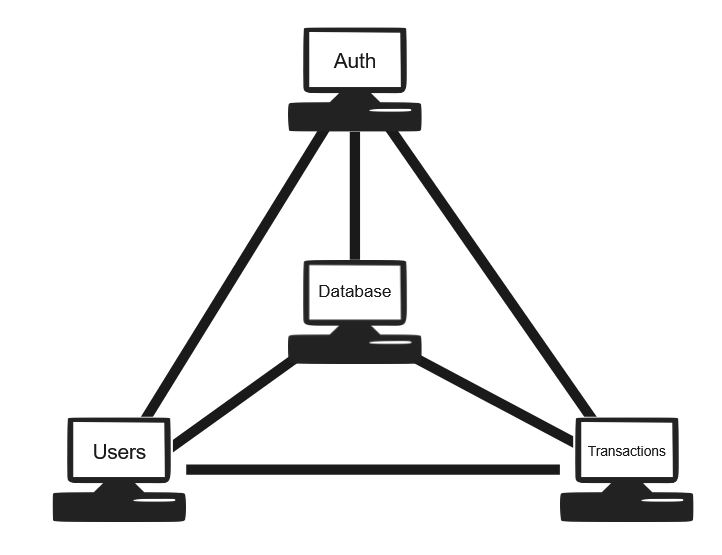
\includegraphics[scale=0.60]{figures/validation.png}
\centering
\end{figure}

In practice, each node is a Raspberry Pi 4 Model B running Ubuntu Server 22.04 and connected to the same Wi-Fi network. Each device is an Erlang node running only the code that pertains to their specific service. All communication is done through Elixir/Erlang primitives for mobility.

Each node has specific responsibilities. The database service handles all persistent data and is the only node whose implementation remains the same in both implementations of the application. It is implemented as a GenServer and supports reading and changing information about users and bank balances. The authentication node basically only has one function that verifies whether a username and password pair is correct. The users node has a function that returns a user's bank balances. Finally, the transactions node has functions for both withdrawing and depositing a certain amount of money into a bank account. In the traditional approach, each of these nodes runs a GenServer that calls their internal functions, while the by-move approach simply lets these functions travel between the nodes.

Each node must carry out some tasks that involve functions from all the nodes. The authentication node must first authenticate a user, then check their bank balance and then withdraws some amount of money. The users node must authenticate a user, then deposits some amount of money. Finally, the transactions node must also authenticate a user, get their balance, and this node will both withdraw from a user and deposit the same amount into a different user's balance. To test the system, each individual action will be performed a certain amount of times, where more actions represent more load on the entire system.

% I think this can go somewhere else.
In the by-move solution we must wait until we are sure we have a function. Not doing this step could result in crashes since the program calls a function that doesn't exist. Here is an example of how this is implemented.

\begin{lstlisting}[language=elixir, caption=Checking and waiting for a function.]
  if !ByMove.have_func?(Transaction,{:get_balance, 2}) do
    ByMove.i_need_func({:get_balance, 2}, nodes, self())
    ByMove.module_wait_for_func(Transaction,{:get_balance, 2}, nodes, self(), [])
  end
\end{lstlisting}

Unless we can be absolutely sure that we have a function at a specific point in time, we must do something like this before calling any function, even ones that originated on the same node.

A variable of interest, and what was measured in each test, was the network flow, or the amount of data in bytes that leaves each of the nodes in the system. This was measured by capturing TCP packets for the duration of the test. It would be expected that as the load on the system increases, the amount of network flow of the by-move solution would be less than that of the traditional solution, since in the traditional approach the amount of data sent is linear to the amount of data that needs to be processed, while in the by-move solution the amount of data sent is constant, corresponding to the size of the AST of the functions being sent.

Three tests were done, one where each action was performed once, 100 times, and 1000 times. We can see the results in the following table.

\begin{table}[!ht]
    \centering
    \caption{Results. All units are in bytes except for the number of actions column.}
    \label{tab:table1}
    \makebox[\linewidth]{
    \begin{tabular}{c|c|c|c|c|c|c}
      \textbf{\# of Actions} & \textbf{Implementation} & \textbf{DB Node} &\textbf{Auth Node} & \textbf{Users Node} & \textbf{Transaction Node} &  \textbf{Total}\\
      \hline
      \multirow{2}{*}{1} & Standard & 8,009 & 4,868 & 4,303 & 5,789 & 22,969\\ % <-- Combining 2 rows with arbitrary with (*) and content 12
                         & By-Move &8,801& 5,783& 5,347& 7,150 & 27,081\\ % <-- Content of first column omitted.
                         \hline
      \multirow{2}{*}{100} &Standard &150,602&136,419&90,212&50,101&427,334 \\ % <-- Combining 2 rows with arbitrary with (*) and content 12
                         & By-Move& 157,383&96,853&88,248&90,274&432,758\\ % <-- Content of first column omitted.
                         \hline
      \multirow{2}{*}{1000} & Standard &1,439,225&1,327,074&877,247&464,351&4,107,897\\ % <-- Combining 2 rows with arbitrary with (*) and content 12
                         & By-Move & 1,497,686&870,045&843,992&847,571&4,059,294\\ % <-- Content of first column omitted.
      \hline
    \end{tabular}
   }
\end{table}

We observe that by 1000 actions, the by-move implementation has an edge over the standard implementation.

